\documentclass[a4paper]{article}
\usepackage{fontspec}
\usepackage{amsmath}
\usepackage{amsfonts}
\usepackage{amssymb}
\usepackage{graphicx}
\usepackage{subcaption}
\usepackage[colorlinks=true,
linkcolor=blue,
citecolor=blue,
urlcolor=blue]
{hyperref}
\usepackage{cleveref}
\usepackage[left=1.00in, right=1.00in, top=1.00in, bottom=1.00in]{geometry}
\usepackage{booktabs}
\usepackage{lmodern}
\title{Introduction to Materials}
\author{Daniel Celis Garza}
\date{\today}
\begin{document}
\maketitle
	\section{Question 1}
	\subsection{a)}
	\subsubsection{i)}
		How many atoms in a BCC unit cell?
		
		\begin{figure}
			\centering
			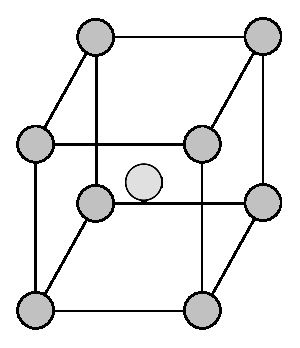
\includegraphics[width=0.33\linewidth]{bcc.eps}
			\caption{BCC unit cell.}
			\label{f:bcc}
		\end{figure}
		2 atoms per unit cell. $1/8$ atom per vertex, $1$ atom in the middle.
		
	\subsubsection{ii)}
		Estimate the density of Chromium (BCC) if the atomic radius, $R = 0.125$ nm, molar mass, $M = 52.0$ g/mol.
		
		\begin{figure}
			\centering
			\begin{subfigure}[b]{0.3\linewidth}
				\centering
				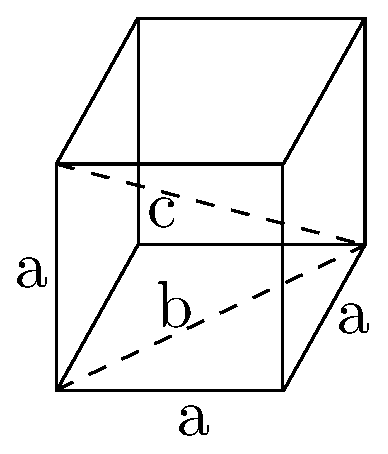
\includegraphics[width=\linewidth]{diag.eps}
				\caption{Cube diagonals.}
				\label{sf:diag}
			\end{subfigure}
			~
			\begin{subfigure}[b]{0.3\linewidth}
				\centering
				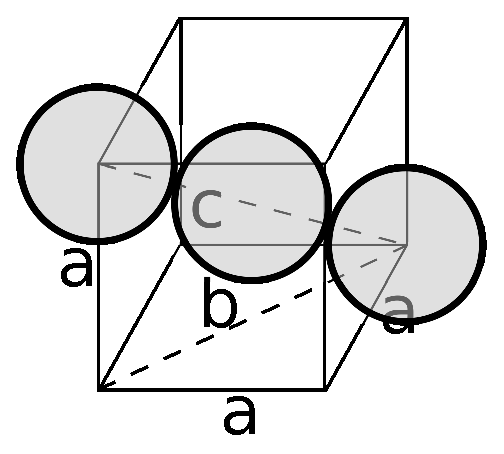
\includegraphics[width=\linewidth]{diag2.eps}
				\caption{Main diagonal (space filling).}
				\label{sf:diag2}
			\end{subfigure}
			~
			\begin{subfigure}[b]{0.3\linewidth}
				\centering
				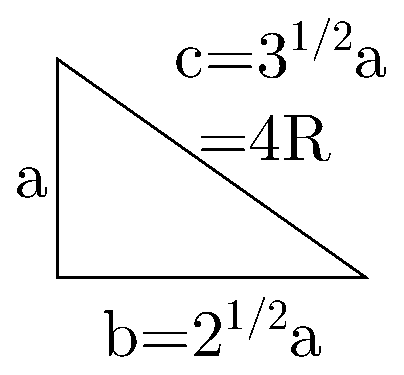
\includegraphics[width=\linewidth]{triag.eps}
				\caption{Diagonal values.}
				\label{sf:diag3}
			\end{subfigure}
			\label{f:diag}
		\end{figure}
		Density,
		\begin{align}
			\rho = m/v~, \label{e:dens}
		\end{align}
		where $m \equiv $ mass and $v \equiv $ volume. From \cref{f:diag} we find,
		\begin{align}
			a &= \dfrac{4}{\sqrt{3}} R \\
			v_{\textrm{unit cell}} &= a^{3} = \left(\dfrac{4}{\sqrt{3}}\right)^{3} R^{3}~, \label{e:volume}
		\end{align}
		The mass of a BCC metal in a unit cell, 
		\begin{align}
			m_{\textrm{unit cell}} = M \times \dfrac{2}{A_{N}}, \label{e:mass}
		\end{align} 
		where $2 \equiv $ number of atoms in a unit cell and $A_{N} \equiv $ avogadro's constant. Substituting \cref{e:volume, e:mass} into \cref{e:dens} we obtain an expression for the density of any BCC metal using values for its unit cell,
		\begin{align}
			\rho = \dfrac{2 \sqrt{3^{3}} M }{4^{3} R^{3} A_{N}}~.
		\end{align}
		Substituting the relevant values we find \cref{se:rho},
		\begin{subequations}
		\begin{align}
			\rho &= \dfrac{2 \sqrt{27} \times 52.0}{4^{3} \left(0.125 \times 10^{-7} \right)^{3} 6.022 \times 10^{23} \textrm{atom/mol}} \dfrac{[\textrm{atom g mol$^{-1}$}]}{[\textrm{atom cm$^{3}$ mol$^{-1}$}]}\\
			     &= 7.18 \textrm{ g/cm$^{3}$} \label{se:rho}\\
			\rho_{\textrm{real}} &= 7.15 \textrm{ g/cm$^{3}$}~.
		\end{align}
		\end{subequations}
		
		\subsection{b)}
		\subsubsection{i)}
		Given, 
		\begin{align}
			v_{1} &= \begin{bmatrix}
					1 & 2 & 3
					\end{bmatrix}\\
			v_{2} &= \begin{bmatrix}
					1 & 1 & -1
					\end{bmatrix}\\
			v_{3} &= \begin{bmatrix}
					1 & 1 & 1
					\end{bmatrix}~.
		\end{align}
		Show $v_{1} \parallel v_{2}$ and $v_{1} \not\parallel v_{3}$.
		
		By the dot product,
		\begin{subequations}		
		\begin{align}
			v_{1} \cdot v_{2} &= \begin{bmatrix}
								1 & 2 & 3
								\end{bmatrix} 
								\begin{bmatrix}
								1\\
								1\\
								-1
								\end{bmatrix}
							    = 1 + 2 - 3 = 0\\
			v_{1} \cdot v_{3} &= \begin{bmatrix}
								1 & 2 & 3
								\end{bmatrix} 
								\begin{bmatrix}
								1\\
								1\\
								1
								\end{bmatrix}
								= 1 + 2 + 3 = 6~.
		\end{align}
		\end{subequations}
	\subsubsection{ii)}
	The zone axis refers to translational invariance between planes. They're described as integer basis vectors such that translations by the basis vector can move any plane to another with the same zone axis. Essentially they are a linear map $f: R^{2} \to R^{2'}$, $f$ being the zone axis. Represented here as the trace of a $3\times3$ matrix.
	\begin{align}
		\begin{bmatrix}
		u & v & w
		\end{bmatrix} &\to 
		\begin{bmatrix}
		u' & v' & w'
		\end{bmatrix}\\
		\begin{bmatrix}
		u & v & w
		\end{bmatrix}
		\begin{bmatrix}
		a & 0 & 0\\
		0 & b & 0 \\
		0 & 0 & c
		\end{bmatrix}
		&=
		\begin{bmatrix}
		u' & v' & w'
		\end{bmatrix}~.
	\end{align}
	\subsubsection{iii)}
	The indices of zone axis can be found by simple vector subtraction of the parallel plane, and multiplying by the smallest factor so all numbers are integer values.
	\begin{align}
		v_{1} - v_{2} = 
		\begin{bmatrix}
		0 & 1 & 4
		\end{bmatrix}~.
	\end{align}
	
	\subsection{c)}
	Cu$_{3}$Au has an FCC lattice. If the collection of atoms is translated to all vertices of the unit cell we obtain an FCC lattice (\cref{f:fcc}).
	\begin{figure}
		\centering
		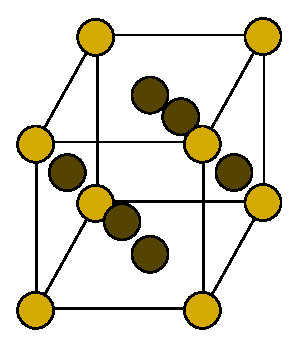
\includegraphics[width=0.33\linewidth]{cu3au.eps}
		\caption{FCC Cu$_{3}$Au unit cell.}
		\label{f:fcc}
	\end{figure}
	\subsection{d)}
	Ni has an FCC unit cell. From \cref{f:fcc} we see that the crystallographic direction for the nearest neighbours are,
	\begin{align}
		\begin{bmatrix}
		\dfrac{1}{2} & \dfrac{1}{2} & 0
		\end{bmatrix},~
		\begin{bmatrix}
		\dfrac{1}{2} & 0 & \dfrac{1}{2}
		\end{bmatrix},~
		\begin{bmatrix}
		0 & \dfrac{1}{2} & \dfrac{1}{2}
		\end{bmatrix},~
	\end{align}
	and the second nearest neighbours,
	\begin{align}
		\begin{bmatrix}
		1 & 0 & 0
		\end{bmatrix},~
		\begin{bmatrix}
		0 & 1 & 0
		\end{bmatrix},~
		\begin{bmatrix}
		0 & 0 & 1
		\end{bmatrix}.
	\end{align}
	\subsection{e)}
	Hexagonal close-packed structures can be represented by translating only two atoms throughout the primitive lattice. \Cref{f:hcp2d} shows the 2D projection of the HCP primitive lattice to illustrate the idea.
	\begin{figure}
		\centering
		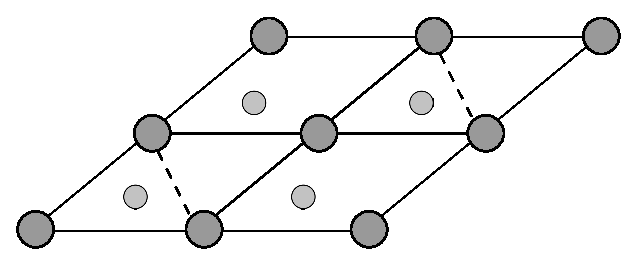
\includegraphics[width=0.33\linewidth]{hcp2d.eps}
		\caption{2D projection of HCP lattice showing how only two atoms need to be translated between lattice points to produce the structure. Smaller atoms lie on planes lower than the bigger ones. Dashed lines represent the non-primitive hexagonal unit cell.}
		\label{f:hcp2d}
	\end{figure}
	
	\section{Question 2}
	For diffraction to occur, the difference in distance travelled by both rays must be an integer multiple of the X-ray wavelength. Otherwise destructive interference will annihilate them both. From \cref{f:xraydiff} we know,
	\begin{subequations}
		\begin{align}
			n \lambda &= AB + BC - AD  \\
			AB &= BC = \dfrac{d}{\sin(\theta)} \\
			AC &= \dfrac{2 d}{\tan(\theta)} \\
			AD &= AC \cos(\theta) = \dfrac{2 d \cos^{2}(\theta)}{\sin(\theta)} \\
			n \lambda &= \dfrac{2 d}{\sin(\theta)} - \dfrac{2 d}{\sin(\theta)} \cos^{2}(\theta) \\
			n \lambda &= \dfrac{2 d}{\sin(\theta)} \left(1 - \cos^{2}(\theta)\right) \\
			n \lambda &= \dfrac{2 d}{\sin(\theta)} \sin^{2}(\theta) \\
			n \lambda &= 2 d \sin(\theta)~.
		\end{align}
	\end{subequations}
	Because we're in cubic symmetry we can use the Euler norm to find the inter planar distance,
	\begin{align}
		d = \dfrac{a}{\sqrt{h^{2} + k^{2} + l^{2}}}~.
	\end{align}
	Ignoring higher frequency harmonics and defining $N = h^{2} + k^{2} + l^{2}$ we arrive at,
	\begin{align}
		\lambda = \dfrac{2a}{\sqrt{N}} \sin(\theta)~.
	\end{align}
	\begin{figure}
		\centering
		\includegraphics[width=0.33\linewidth]{bragg.eps}
		\caption{Schematic of X-ray diffraction.}
		\label{f:xraydiff}
	\end{figure}
	\subsection{b)}
	The structure factor gives information on the amplitudes and phase of the diffracted beams,
	\begin{align}
		F_{hkl} = \sum\limits_{i=1}^{N} f_{i} \exp\left[ -2 \pi i (h x_{i} + k y_{i} + l z_{i}) \right]~,
	\end{align}
	where $i$ represents an atom, $x_{i},~ y_{i},~ z_{i}$ are the coordinates of the basis atoms that comprise the primitive unit cell, and $h,~ k,~ l$ are a plane's miller indices, and $f_{i}$ is the scattering factor for the $i$'th atom. For certain planes, the structure factor vanishes completely and as a result, the intensity of the refracted beam is zero for such planes. This leads to a systematic absence of planes, and therefore the selection rules as seen in the lecture course.
	
	\subsection{c)}
	Using an X-ray $\lambda = 0.1524$ nm, on a cubic crystal powder.
	\subsubsection{i)}
	\Cref{t:diff} shows the refracting planes.
	\begin{table}
		\centering
		\caption{Diffraction table with crystal planes.}
		\label{t:diff}
		\begin{tabular}{cccccc}
			\toprule
			$2\theta$ & $\theta$ & $\sin^{2}\theta$ & $N = \sin^{2}\theta/R$ & $h,~ k,~ l$ & $ R = \sin^{2}\theta/N $\\
			\midrule
			$28.2$ & $14.1$  & $0.059$ & $3$  & $1,~1,~1$ & $ 0.0198 $ \\
			$32.7$ & $16.35$ & $0.079$ & $4$  & $0,~0,~2$ & $ 0.0198 $ \\
			$46.9$ & $23.45$ & $0.158$ & $8$  & $0,~2,~2$ & $ 0.0198 $ \\
			$55.6$ & $27.8$  & $0.218$ & $11$ & $1,~1,~3$ & $ 0.0198 $ \\
			$58.3$ & $29.15$ & $0.237$ & $12$ & $2,~2,~2$ & $ 0.0198 $ \\
			$68.4$ & $34.2$  & $0.316$ & $16$ & $0,~0,~4$ & $ 0.0198 $ \\
			$75.6$ & $37.8$  & $0.376$ & $19$ & $1,~3,~3$ & $ 0.0198 $ \\
			$77.9$ & $38.95$ & $0.395$ & $20$ & $0,~2,~4$ & $ 0.0198 $ \\
			$87.1$ & $43.55$ & $0.475$ & $24$ & $2,~2,~4$ & $ 0.0198 $ \\
			\bottomrule
		\end{tabular}
	\end{table}
	\subsubsection{ii)}
	The lattice parameter $a$, is given by,
	\begin{subequations}
		\begin{align}
			a &= \dfrac{\lambda}{2 \sqrt{R}}\\
			  &= \dfrac{0.1524}{2 \sqrt{0.0198}} = 0.5404 \textrm{ nm}~.
		\end{align}
	\end{subequations}
	
	\section{Question 3}
	\subsection{a)}
	The root mean squared free path is given by,
	\begin{align}
		x_{rms} = \sqrt{D t}~,\label{e:rms}
	\end{align}
	where $D \equiv $ diffusivity and $t \equiv$ time. Assuming the diffusivity to be an activated process we have,
	\begin{align}
		D = D_{0} \exp\left(-\dfrac{Ea}{RT}\right)~,\label{e:diff}
	\end{align}
	where $Ea \equiv$ activation energy, $R \equiv $ ideal gas constant and $T \equiv$ temperature. Plugging \cref{e:diff} into \cref{e:rms},
	\begin{align}
		x_{rms} = \sqrt{D_{0} \exp\left(-\dfrac{Ea}{RT}\right) t}~.\label{e:rmsdiff}
	\end{align}
	
	First we need to find $D_{0}$ for the known scenario $x_{rms} = 0.5 \textrm{ mm},~ T = 293.15 \textrm{ K},~ Ea = 30 \text{ kJ},~ R = 8.314 \text{ J mol$^{-1}$ K$^{-1}$ }$,
	\begin{subequations}
	\begin{align}
		D_{0} &= \dfrac{0.5^{2} \exp\left(\dfrac{30 \times 10^{3}}{8.314 \times 293.15}\right) }{30} \dfrac{\textrm{[mm$^2$]}}{\textrm{[min]}}\\
			  &= 1847.28 \textrm{ mm$^2$ min$^{-1}$}.~
	\end{align}
	\end{subequations}
	We then solve for $t$ at $T = 353.15 \textrm{ K}$,
	\begin{subequations}
	\begin{align}
		t &= \dfrac{0.5^{2} \exp\left(\dfrac{30 \times 10^{3}}{8.314 \times 353.15}\right) }{1847.28} \dfrac{\textrm{[mm$^2$]}}{\textrm{[mm$^2$ min$^{-1}$]}}\\
		  &= 3.706 \textrm{ min}
	\end{align}
	\end{subequations}
	\subsection{b)}
	Edge dislocations are concerted movements of lines of atoms perpendicular to the Burger's vector. As a result, the dislocation moves parallel to the vector because subsequent perpendicular lines of atoms become displaced. Screw dislocations are concerted movements of lines of atoms parallel to the Burgers vector. As more parallel lines of atoms become displaced, the dislocation moves perpendicular to the Burgers vector. \Cref{f:dis} shows both dislocation types and their movement.
	\begin{figure}
		\centering
		\begin{subfigure}[b]{0.45\linewidth}
			\centering
			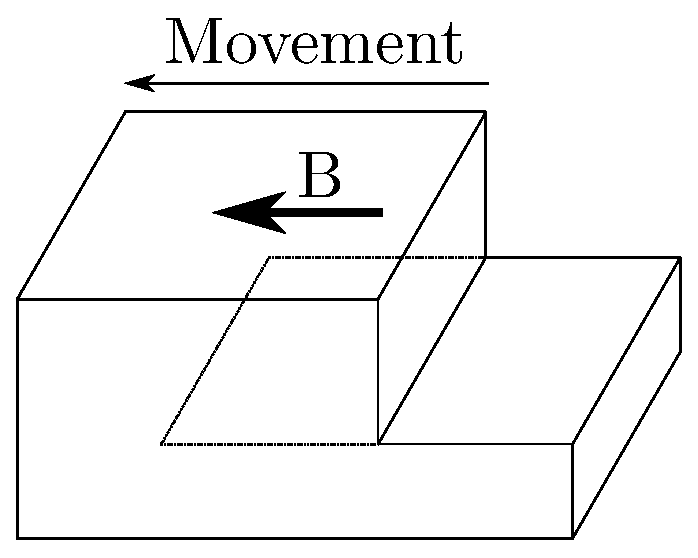
\includegraphics[scale=0.5]{edgedis.eps}
			\caption{Edge dislocation.}
		\end{subfigure}
		~
		\begin{subfigure}[b]{0.45\linewidth}
			\centering
			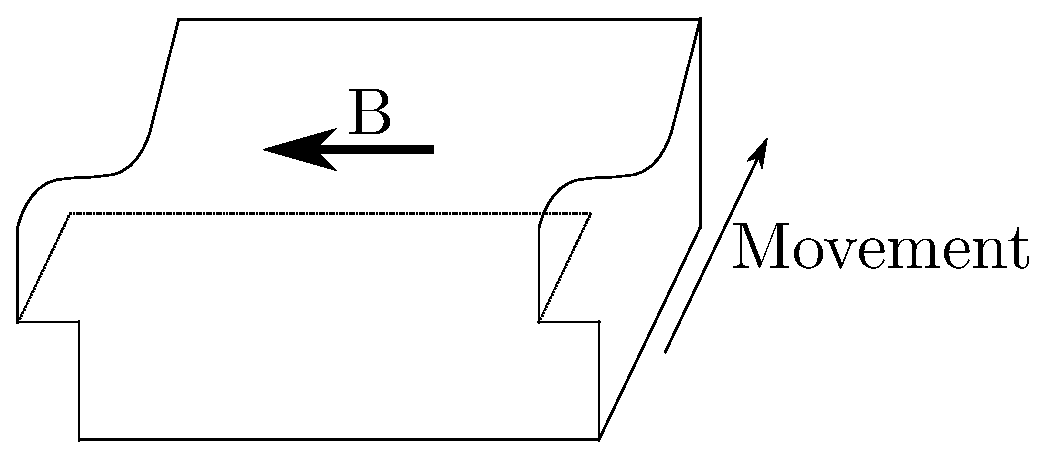
\includegraphics[scale=0.5]{screwdis.eps}
			\caption{Screw dislocation.}
		\end{subfigure}
		\caption{Dislocation types. Burger's vector is denoted by $B$.}
		\label{f:dis}
	\end{figure}
	\subsection{c)}
	The dislocation can be decomposed as follows,
	\begin{align}
		\dfrac{a}{2}
		\begin{bmatrix}
		1 & \overline{1} & 0 
		\end{bmatrix}
		\to
		\dfrac{a}{6}
		\begin{bmatrix}
		2 & \overline{1} & \overline{1} 
		\end{bmatrix}
		+
		\dfrac{a}{6}
		\begin{bmatrix}
		\overline{1} & 2 & \overline{1} 
		\end{bmatrix}~.
	\end{align}
	The dislocation energy is proportional to the modulus of each dislocation. A single dislocation will split into two partial dislocations if the energy of the two partials plus the stacking fault energy, $E_{s}$, is less than the energy of a full dislocation,
	\begin{subequations}
	\begin{align}
		\dfrac{a^{2}}{4} 
		\begin{bmatrix}
			1 & -1 & 0 
		\end{bmatrix}
		\begin{bmatrix}
		1\\ -1\\ 0 
		\end{bmatrix} 
		&\overset{?}{=}
		\dfrac{a^{2}}{36}
		\begin{bmatrix}
		2 & -1 & -1
		\end{bmatrix}
		\begin{bmatrix}
		2 \\ -1 \\ -1
		\end{bmatrix}
		+
		\dfrac{a^{2}}{36}
		\begin{bmatrix}
		-1 & 2 & -1
		\end{bmatrix}
		\begin{bmatrix}
		-1\\ 2 \\ -1
		\end{bmatrix}
		+ E_{s}\\
		\dfrac{a^{2}}{2} &\overset{?}{=} \dfrac{a^{2}}{3} + E_{s}~.
	\end{align}
	\end{subequations}
	The partial dislocations form an angle of $\frac{2}{3}\pi$ rad.
\end{document}